\documentclass{article}

% if you need to pass options to natbib, use, e.g.:
%     \PassOptionsToPackage{numbers, compress}{natbib}
% before loading neurips_2018

% ready for submission
% \usepackage{neurips_2018}

% to compile a preprint version, e.g., for submission to arXiv, add add the
% [preprint] option:
%     \usepackage[preprint]{neurips_2018}

% to compile a camera-ready version, add the [final] option, e.g.:
\usepackage[final,nonatbib]{nips_2018}

% to avoid loading the natbib package, add option nonatbib:
%     \usepackage[nonatbib]{neurips_2018}

\usepackage[utf8]{inputenc} % allow utf-8 input
\usepackage[T1]{fontenc}    % use 8-bit T1 fonts
\usepackage{hyperref}       % hyperlinks
\usepackage{url}            % simple URL typesetting
\usepackage{booktabs}       % professional-quality tables
\usepackage{amsfonts}       % blackboard math symbols
\usepackage{nicefrac}       % compact symbols for 1/2, etc.
\usepackage{microtype}      % microtypography
\usepackage{graphicx}
\usepackage{siunitx}

% bibliography stuff
\PassOptionsToPackage{%
  backend=biber,bibencoding=utf8, %instead of bibtex
  %backend=bibtex8,bibencoding=ascii,%
  language=auto,%
  % style=nature,%
  style=authoryear-comp, % Author 1999, 2010
  %bibstyle=authoryear,dashed=false, % dashed: substitute rep. author with ---
  %sorting=nyt, % name, year, title
  maxbibnames=3, % default: 3, et al.
  backref=true,%
  natbib=false % natbib compatibility mode (\citep and \citet still work)
}{biblatex}
\usepackage{biblatex}
\addbibresource{bibliography.bib}

\title{Crabsort: spike-sorting for small circuit networks}

\author{%
  Alec Hoyland \\
  Center for Systems Neuroscience \\
  Boston University \\
  Boston, MA 02215 \\
  \texttt{entropyvsenergy@posteo.de} \\
  \And
  Cosmo Guerini \\
  Department of Biology and Volen National Center for Complex Systems \\
  Brandeis University \\
  Waltham, MA 02453 \\
  \texttt{machinelearning@cosmo.red}
}

\begin{document}

\maketitle

\begin{abstract}
  Crabsort.
\end{abstract}

\section{Introduction}

Electrophysiological recording by extracelullar electrode is one of the simplest and most reliable
methods for recording local electrical activity around the electrode tip.
Action potentials produce characteristic voltage deflections, known as a spike waveform.
The extracellular recordings take the form of voltage time series, with one waveform for each electrode,
from which spikes must be identified, as well as from which cell the spike originates \autocite{quirogaSpikeSorting2012}.
The first task is well-studied, and can be managed effectively by high-pass filtering and counting threshhold crossings \autocite{rossantSpikeSortingLarge2016, quirogaSpikeSorting2012}.
However, it is extremely difficult to tell by eye which spikes originate from which cells.
In larger networks with up to 1,000 simultaneous recordings, algorithms exist which can cluster
based on PCA, SVD, and stochastic k-means matching \autocite{pachitariuKilosortRealtimeSpikesorting2016, rossantSpikeSortingLarge2016}.

In smaller networks, of about 30 cells, where each cell is named and well-studied,
these algorithms break down. With paucity of data and similarity between waveforms of differing cell types,
it is not feasible to use algorithms designed for large multi-channel recordings on smaller circuit data.
Furthermore, methods such as Granger causality can report spurious causal relationships
if the network is strongly oscillatory \autocite{kisperskyFunctionalConnectivityRhythmic2011}.
One solution is to use a mixed linear point process model \autocite{gerhardSuccessfulReconstructionPhysiological2013a},
but this strategy is not extensible to unknown systems, or for use with unlabeled data.

Another strategy, implemented in the software package \texttt{crabsort} (S. Gorur-Shandilya \textit{et al.}, unpublished),
uses pre-sorted data to train a neural network model which can automatically sort the remaining data.
Briefly, this process involves dimensionally-reducing the spike trains to a 2-dimensional manifold
and manually clustering a subset of the data.
A neural network is trained on this dataset to identify which spikes belong to which clusters,
where each cluster is a different neuron.

We extend the \texttt{crabsort} toolkit to include several backends implementing
fast Fourier transform-accelerated interpolation-based t-SNE (FIt-SNE) \autocite{lindermanFastInterpolationbasedTSNE2019, vandermaatenAcceleratingTSNEUsing2014}
and uniform manifold approximation and projection \autocite{mcinnesUMAPUniformManifold2018}.

\section{Crabsort}

\texttt{crabsort} is a toolkit for visualizing and sorting electrophysiological data.
Its name originates in its use on electrophysiological data from the stomatogastric ganglion in crustaceans.

Raw electrophysiological data are loaded into MATLAB (Mathworks, Newton, MA) and spikes are found using the built-in peak finding algorithm
with parameters that can be adjusted in real-time.
The training data typically consists of less than 1 percent of the total data to be spike-sorted.

Snippets around each spike waveform are taken.
The membrane potential at each time step is counted as the value in a different dimension,
so that the number of dimensions is usually around 70.

The data are then dimensionally-reduced to a 2-dimensional manifold.
This is one of the most crucial steps, as the dimensional reduction method determines the spatialization of the clusters
and therefore the representativeness of the training data given to the neural network.
The choice of dimensionality reduction algorithm, along with the noise in the data
and distinguishability of the classifications (different neurons from whence the spike originated)
determine the separation of clusters in the low-dimensional space.

A neural network consisting of two fully-connected layers, interspersed with reLU layers,
is trained on the clustered data.
A layer with a 10 percent dropout rate leads to a softmax-activated classification layer.

After training, \texttt{crabsort} can be used to classify the remaining spikes in the dataset.

If the spike does not clearly fit into one of the classes, \texttt{crabsort} flags it.
If spikes are manually reclassified after viewing the prediction, \texttt{crabsort} retrains the network to encompass those new data.

\subsection{Aims of this project}

We add to the extant \texttt{crabsort} framework,
by extending the dimensionality reduction options beyond naive PCA and t-SNE.
We implement a faster and more accurate version of t-SNE that uses fast-Fourier transform interpolation and parallelized approximate nearest neighbors,
as well as uniform manifold approximation and projection, a very new dimensionality reduction method that is very accurate for subsets of data.

\subsection{Current dimensionality reduction algorithms}

Currently there are three dimensionality-reduction algorithms implemented in \texttt{crabsort}.
The first separates by spike amplitude, which can sometimes be sufficient.
The second uses a naive principle component analysis (PCA) algorithm.
PCA is an eigenvector-based multivariate analysis that linearly transforms a dataset onto
orthogonal principle components which account for as much variance in the data as possible.
It is a linear transformation, and is fast to use, making PCA a popular first step in exploratory data visualization.
Unfortunately, it performs worse at clustering than more recently-developed algorithms.

\texttt{crabsort} also implements t-distributed stochastic neighborhood embeddings (t-SNE),
a type of k-nearest dimensionality reduction algorithm \autocite{vandermaatenAcceleratingTSNEUsing2014}.
t-SNE first computes the conditional probabilities that are proportional to the similarity of each data point.
In the original algorithm, Gaussian kernels are used with the Euclidean distance.
The probability of $x_j$ conditioned on $x_i$ indicates the probability
that $x_j$ would be chosen as a neighbor to $x_i$,
if neighbors were picked in proportion to their probability density under a Gaussian distribution centered at $x_i$.
The bandwidth of the Gaussian kernels (i.e. the variance) is set so that
the perplexity of the conditional distribution equals a predefined hyperparameter value.
Student's t-distribution is used in the low-dimensional representation to measure similarity,
which is compared to the high-dimensional conditional distributions
by minimizing the Kullback-Leibler divergence between the two, by gradient descent.
t-SNE provides much better clustering than PCA, but is much slower, acting in $\mathcal{O}(n^2)$ time.

\section{New dimensionality reduction algorithms}

Since dimensionality reduction is crucial to generating an accurate training dataset,
we implement backends for two improved dimensionality reduction algorithms: FIt-SNE and UMAP.

Since both the FIt-SNE and UMAP wrappers create structs which contain modifiable parameters,
we modify the \texttt{crabsort} framework to expose plugin object parameters,
for real-time tuning of algorithm parameters to better cluster the data.

\subsection{FIt-SNE}

The first, fast Fourier transform-interpolated t-SNE (FIt-SNE)
provides accelerated t-SNE on $\mathcal{O}(n)$.
Common implementations of t-SNE use the Barnes-Hut approximation to simplify the n-body problem
which must be solved during optimizing the embedding, yielding time-complexity $\mathcal{O}(n \log n)$ \autocite{vandermaatenAcceleratingTSNEUsing2014}.
\cite{lindermanFastInterpolationbasedTSNE2019} interpolate an equispaced grid
rather than compute the repulsive forces in the n-body problem directly.
Computing the objective function amounts to performing a convolution over the grid.
Since the grid is translation-invariant with respect to the interpolating spline functions,
and the matrix associated with the convolution is Toeplitz,
the convolution can be simplified to multiplication in the Fourier domain,
by taking the fast Fourier transform (FFT).

FIt-SNE comes equipped with a MATLAB wrapper that runs the compiled C-code as a MEX file.
We improve the wrapper by through minor speed improvements,
and implement FIt-SNE as a dimensionality reduction plugin for \texttt{crabsort}.

\subsection{UMAP}

In addition, instead of taking k-nearest neighbors,
FIt-SNE uses an approximate nearest-neighbors algorithm, \texttt{ANNOY} \autocite{bernhardssonApproximateNearestNeighbors2019},
which can take advantage of multithreading for a speed increase.
FIt-SNE results in time-complexity $\mathcal{O}(n \log n)$,
but converges 15-30x times faster than the Barnes-Hut accelerated t-SNE implementation.

Like FIt-SNE, uniform manifold approximation and projection (UMAP) \autocite{mcinnesUMAPUniformManifold2018}
is based on a k-nearest neighbors algorithm, however unlike t-SNE, UMAP is not stochastic.
It relies on three core assumptions:

\begin{itemize}
  \item The data are uniformly distributed on a Riemannian manifold.
  \item The Riemannian metric is locally constant (or can be approximated as such).
  \item The manifold is locally connected.
\end{itemize}

While the theoretical underpinnings are satisfactory for any fuzzy simplicial sets,
the algorithm is best implemented over a weighted graph.
The k-nearest neighbors weighted graph can be computed by any suitable algorithm.
UMAP then performs spectral clustering on the Laplacian matrix constructed from the graph.
Optimization of the fuzzy simplicial set cross entropy follows to optimize the embedding.
UMAP is stable under subsampling and must faster than even FIt-SNE,
though the clustering is more opaque, and therefore sometimes less desirable than PCA or t-SNE.
Furthermore, UMAP is deterministic and therefore allows new data to be mapped to the low-dimensional space
without recomputing the entire embedded representation.

Since UMAP is written in Python, we used \texttt{condalab} and a UMAP wrapper for MATLAB
to configure a virtual environment for use with \texttt{crabsort}.

\section{Benchmarking}

Data were collected from the stomatogastric ganglion of \textit{Cancer borealis} crabs
by Daniel Powell in the Marder Laboratory at Brandeis University.
Electrophysiological recordings were taken at a 44.4 kHz sample frequency,
and stored in multiple \texttt{.abf} files.
The dataset used for benchmarking, \texttt{901-046}, was segmented into 126 files.
The first of these files was used for clustering and training the neural network.

180 spikes were found using the \texttt{findpeaks} algorithm
and 947 time steps were taken around each spike.

\begin{figure}
  \centering
  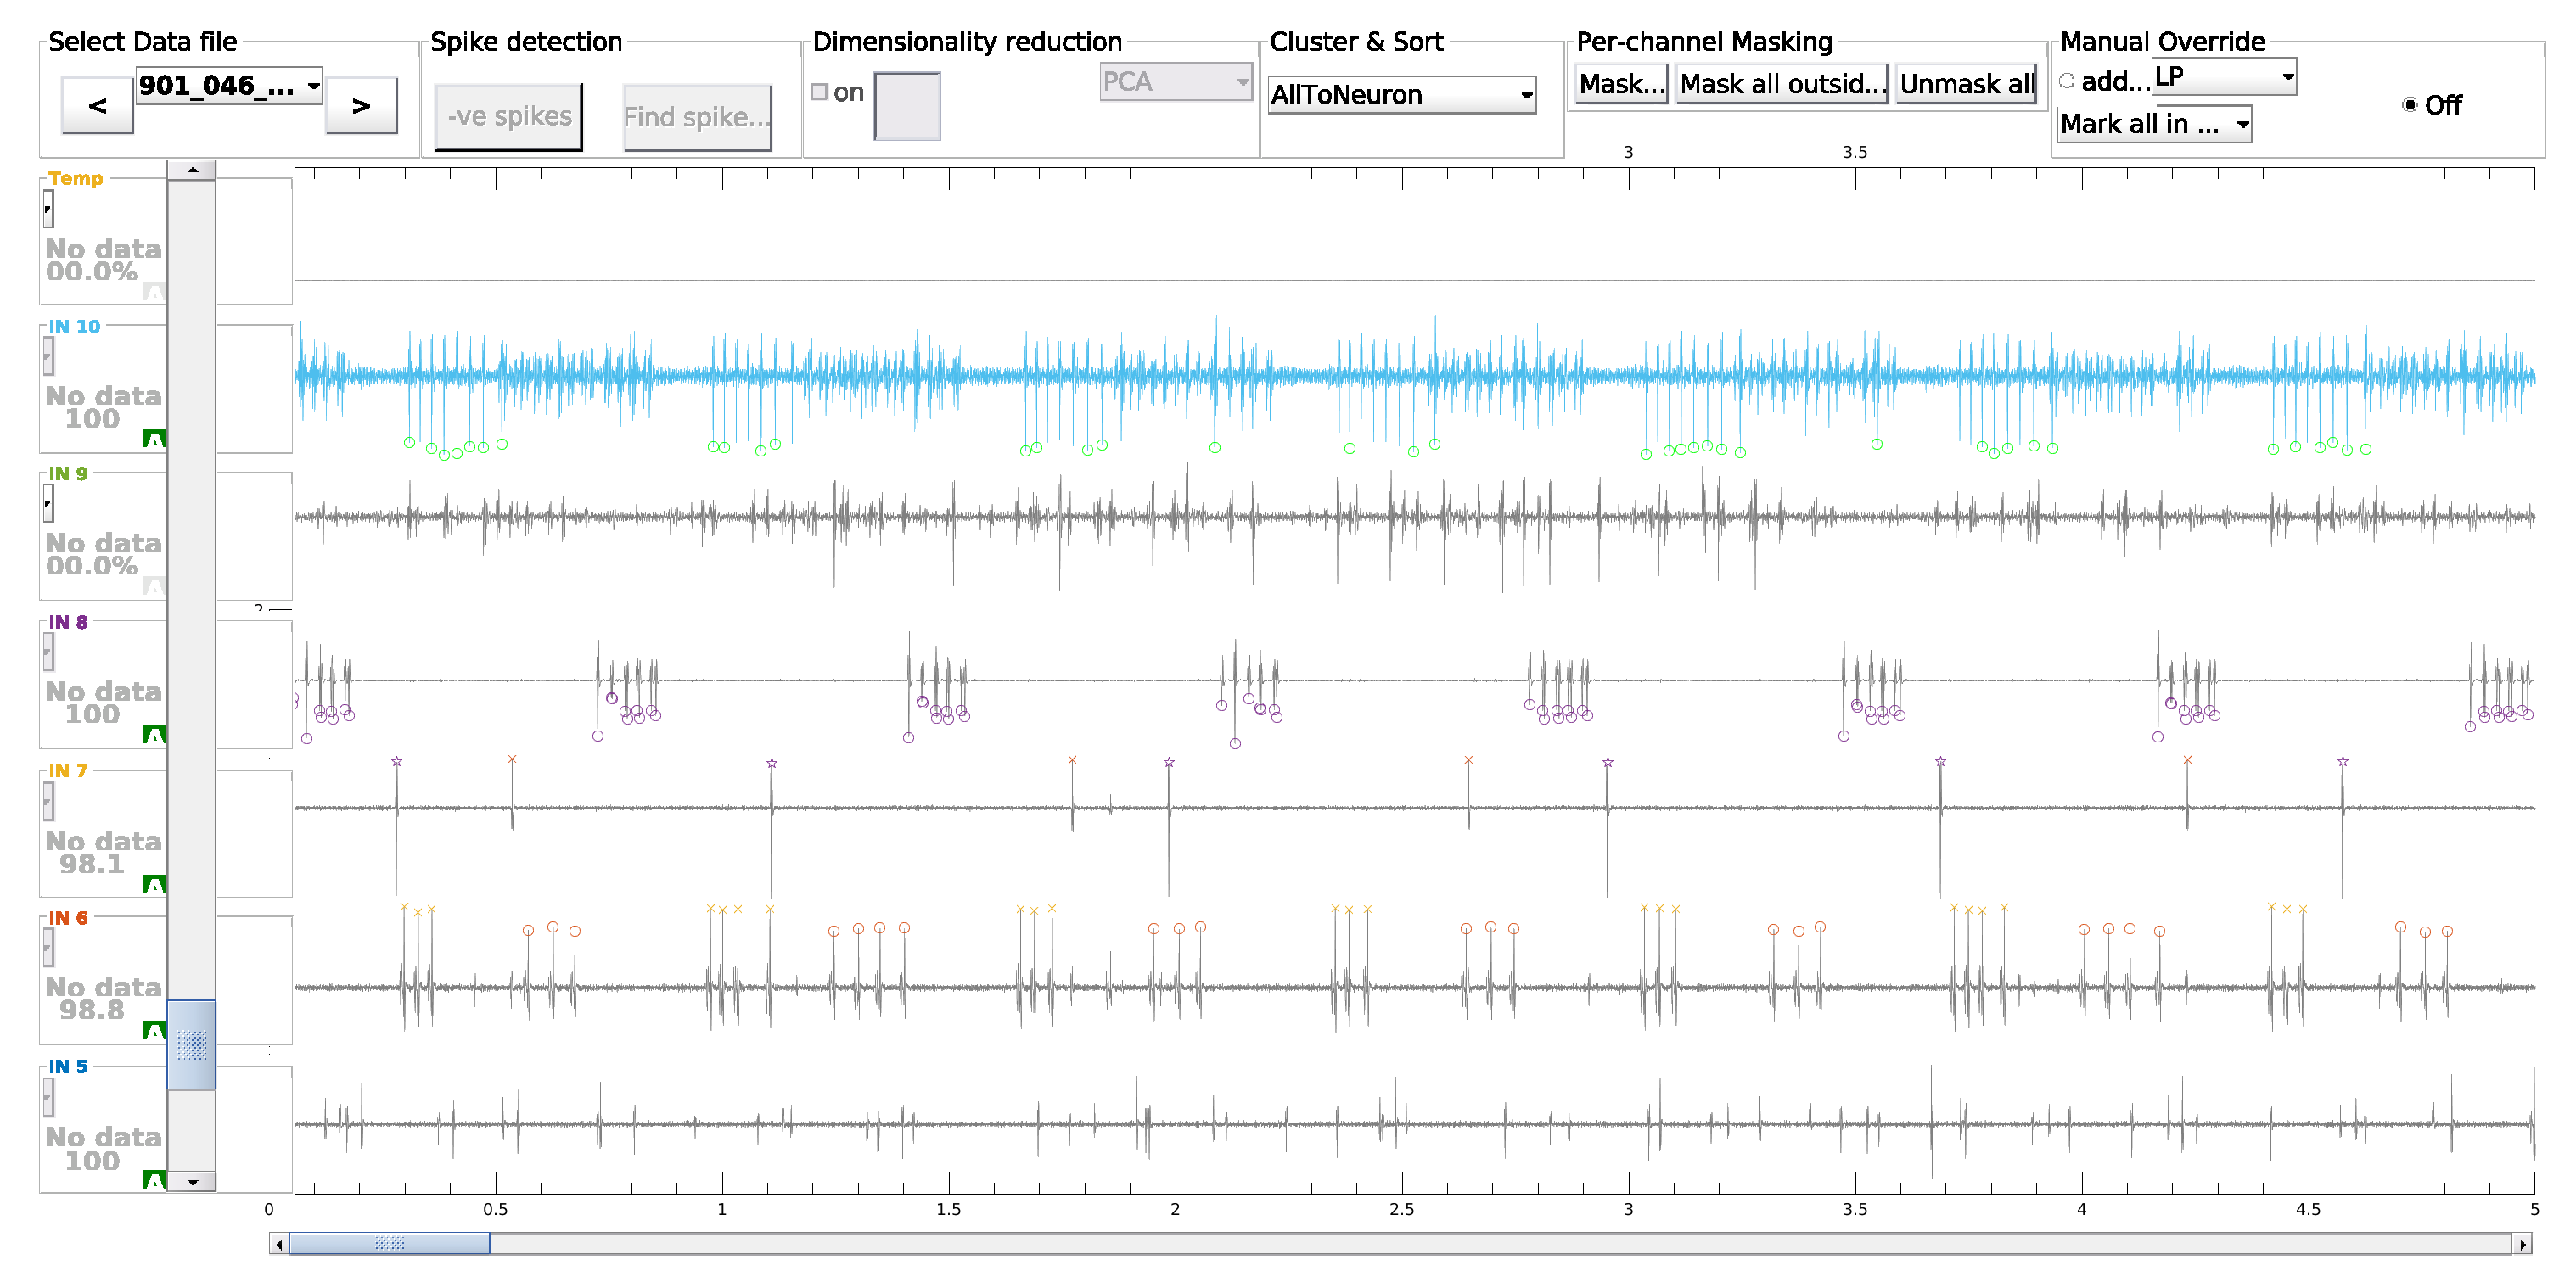
\includegraphics[width=\textwidth]{gfx/crabsort.eps}
  \caption{Snapshot of the \texttt{crabsort} GUI. The top trace was used for benchmarking. Spikes are denoted by circles.}
  \label{fig:crabsort}
\end{figure}

Four dimensionality-reduction schemes were tested: PCA, t-SNE, FIt-SNE, and UMAP.
PCA performs the worst, as it can only account for linear combinations.
t-SNE and FIt-SNE are almost indistinguishable, modulo randomness.
The long chains that appear in the UMAP-reduced presentation are a result of
the simplicial complexes used to construct the topological space.

\begin{figure}
  \centering
  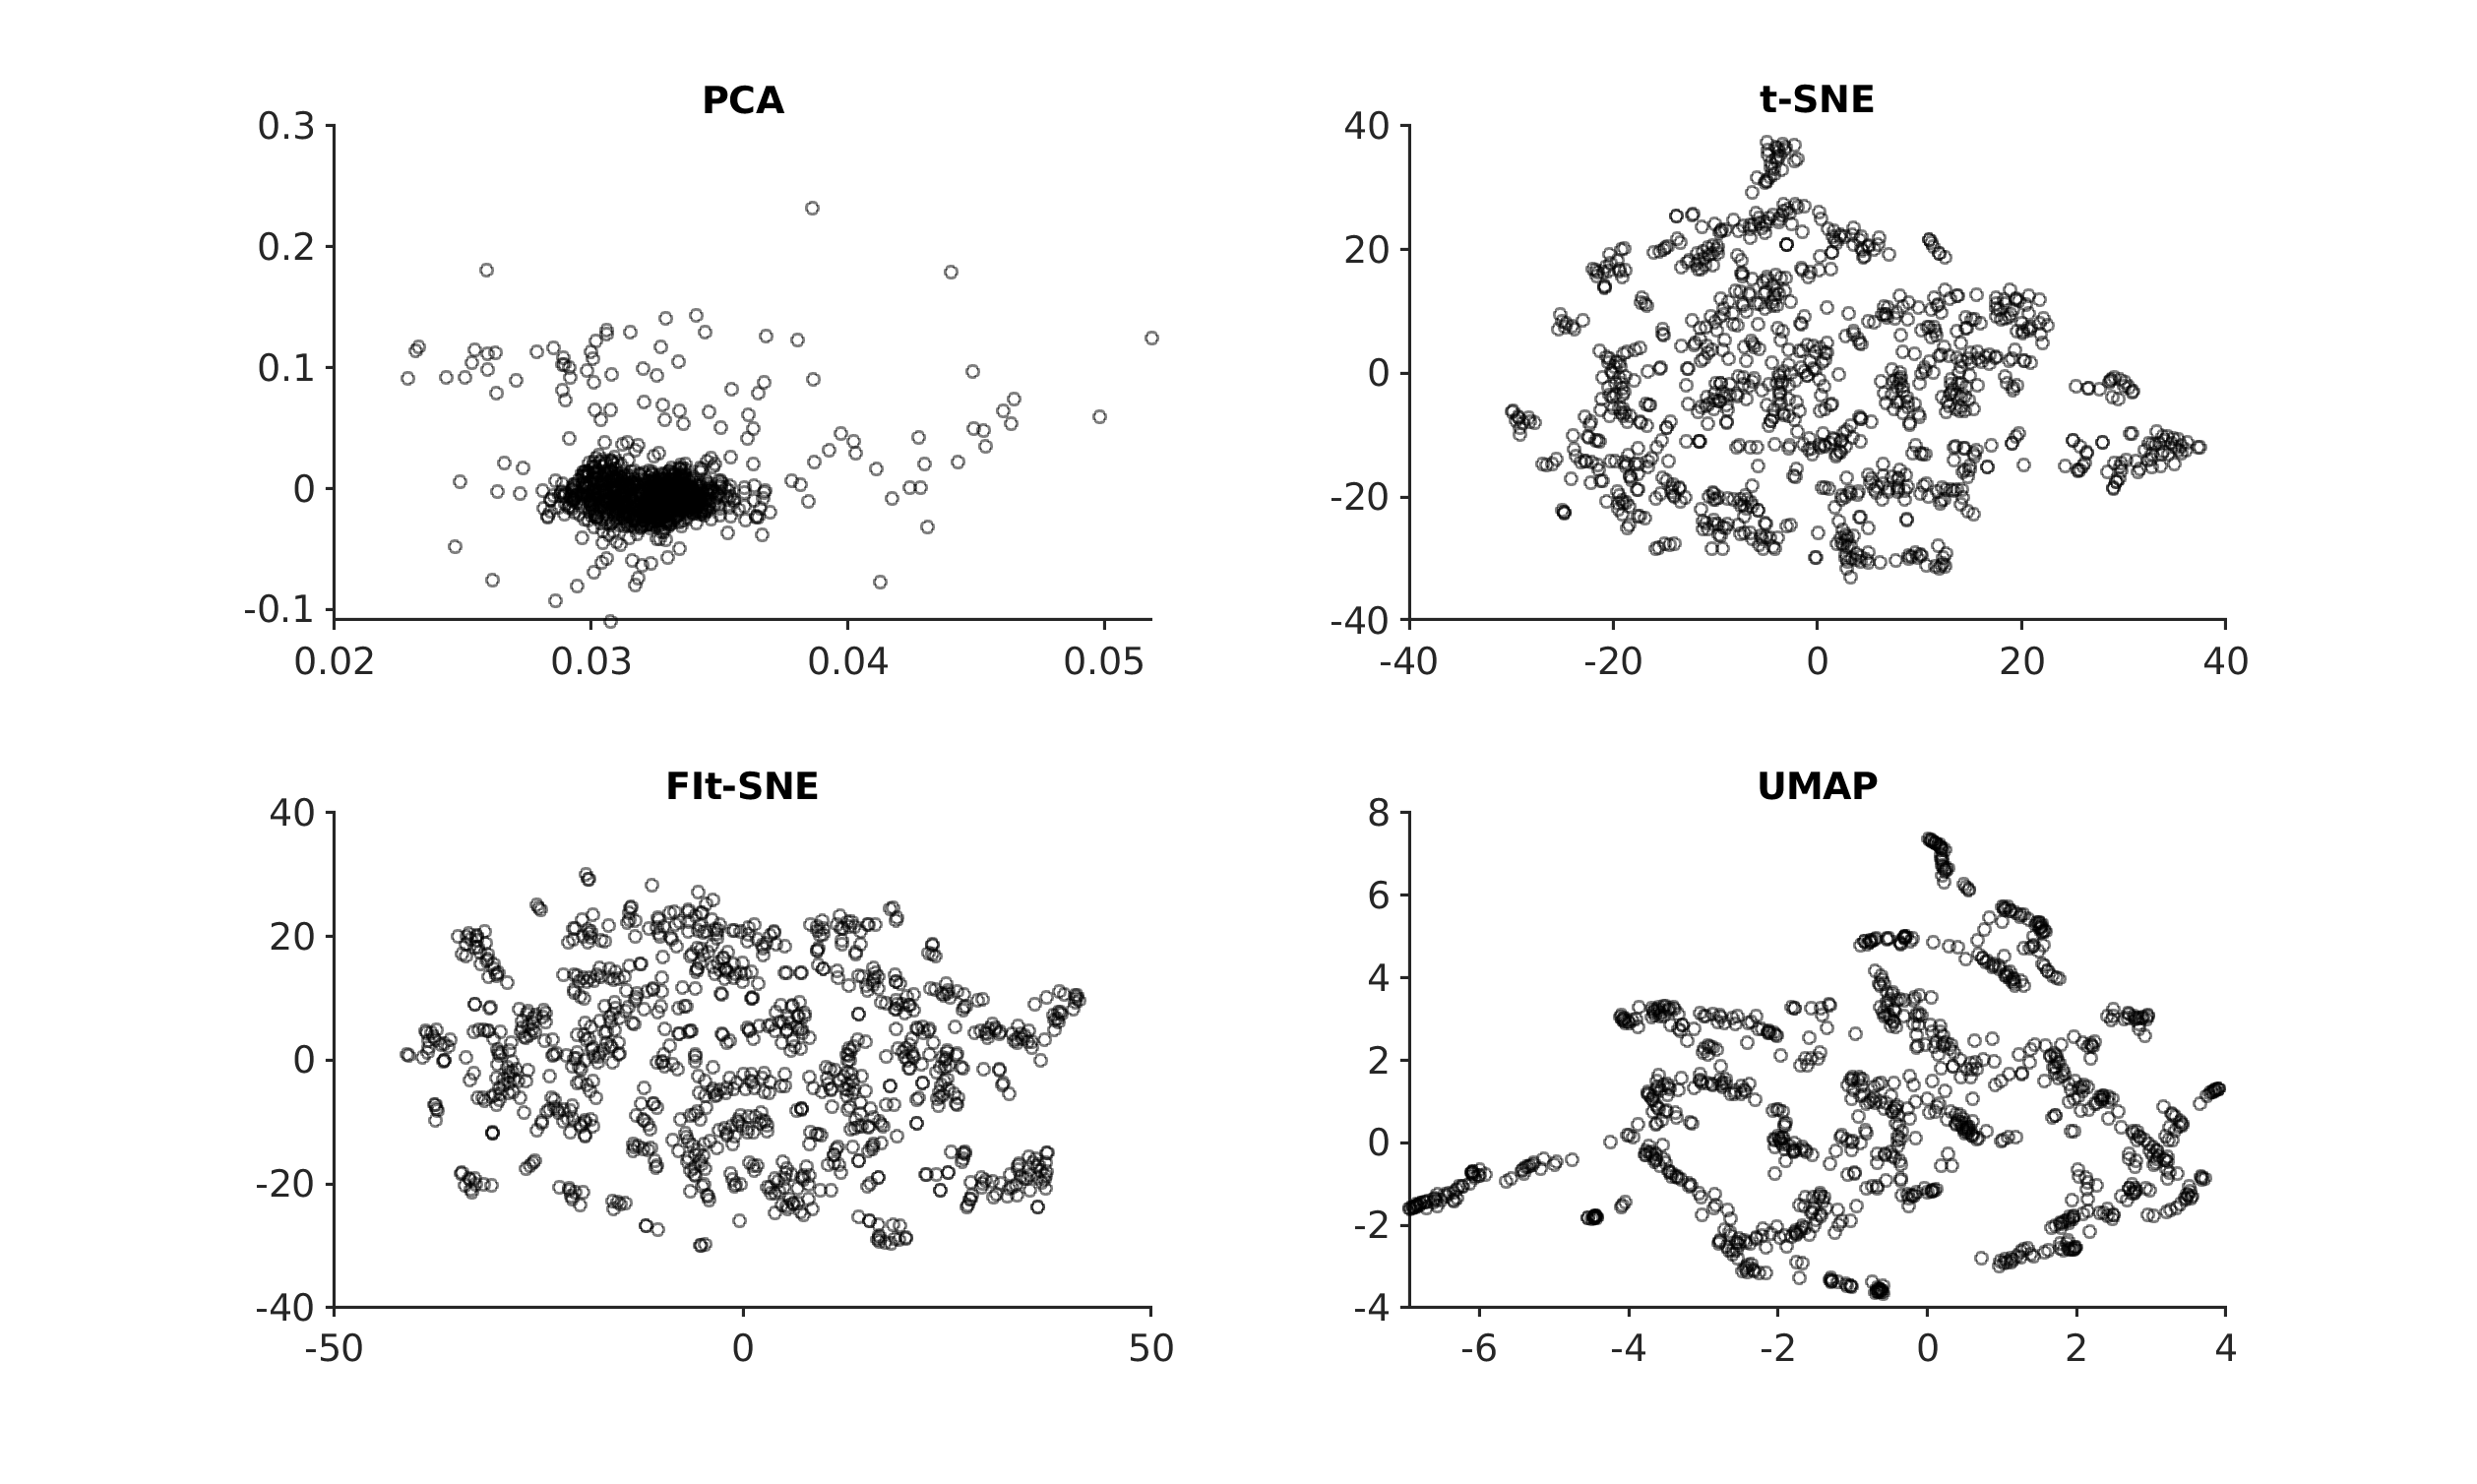
\includegraphics[width=\textwidth]{gfx/dim-red.eps}
  \caption{Four dimensionality-reduction schemes run on the same data.}
  \label{fig:dim-red-comparison}
\end{figure}

Surprisingly, FIt-SNE performed terribly in time benchmarking.
We suspect this is due to the more rigorous optimization algorithm used
to determine the best t-SNE fit.
For example, using the ANNOY library for the approximate k-nearest-neighbors
search was parallelized, and took only 0.037 s with $k=90$.
The algorithm terminated the gradient descent optimization after 1,000 iterations.
Though FIt-SNE should be theoretically faster than t-SNE, for a small dataset,
it proves to be much slower without a significant increase in cluster separation.

UMAP performed as well as promised, acting in a competitive amount of time with t-SNE,
and proved to be the best algorithm among the four tested for this particular application.

\begin{table}
  \caption{Time elapsed during dimensionality reduction.}
  \label{tbl:dim-red-time}
  \centering
  \begin{tabular}{lS}
    \toprule
    Algorithm Name     & Time~Elapsed~(s) \\
    \midrule
    PCA     & 0.0228 \\
    t-SNE   & 5.2076 \\
    FIt-SNE & 21.3535 \\
    UMAP    & 4.5879 \\
    \bottomrule
  \end{tabular}
\end{table}

\subsubsection*{Acknowledgments}

Thank you to Dustin Clark at Research Computing Services, Boston University,
for his help debugging Python-MATLAB compatibility,
and to Srinivas Gorur-Shandilya at Brandeis University,
for helming the \texttt{crabsort} project.
%
% \section*{References}
%
% \medskip
%
% \small

\printbibliography

\end{document}
